\documentclass[class=article, crop=false]{standalone}
\usepackage[subpreambles=true]{standalone}
\usepackage{import}
%%\usepackage{booktabs}
%\usepackage{tikz}

%\usepackage[utf8]{inputenc}
\usepackage[subpreambles=true]{standalone}
\usepackage{import}
\usepackage{pgfplots}
\pgfplotsset{compat=newest}
\usepgfplotslibrary{groupplots}
\usepgfplotslibrary{dateplot}
\usepackage{caption}
\usepackage{subcaption}
\usepackage{graphicx}
\usepackage{amsmath}
\usepackage{amssymb}
\usepackage[parfill]{parskip}
\usepackage{float}

% \usepackage{pgfplots}
% \usetikzlibrary{pgfplots.groupplots}
% \pgfplotsset{compat=1.9,height=0.3\textheight,legend cell align=left,tick scale binop=\times}
% \pgfplotsset{grid style={loosely dotted,color=darkgray!30!gray,line width=0.6pt},tick style={black,thin}}
% \pgfplotsset{every axis plot/.append style={line width=0.8pt}}
%
% \usepgfplotslibrary{external}
% % Für die Verwendung von 'external' müssen die folgenden Anpassungen in Abhängigkeit der
% % LaTeX Distribution durchgeführt werden:
%
% % fuer Texlive: pdflatex.exe -shell-escape -synctex=1 -interaction=nonstopmode %.tex
% \tikzexternalize[shell escape=-shell-escape]   % fuer TeXLive
%
% % fuer MikTeX:  pdflatex.exe -enable-write18 -synctex=1 -interaction=nonstopmode %.tex
% %\tikzexternalize[shell escape=-enable-write18] % fuer MikTex
%
%
%
% \tikzsetexternalprefix{graphics/pgfplots/} % Ordner muss ev. zuerst haendisch erstellt werden


\begin{document}

\section{Hardware}\label{sec:hardware}

\begin{figure}[H]
 \centering
 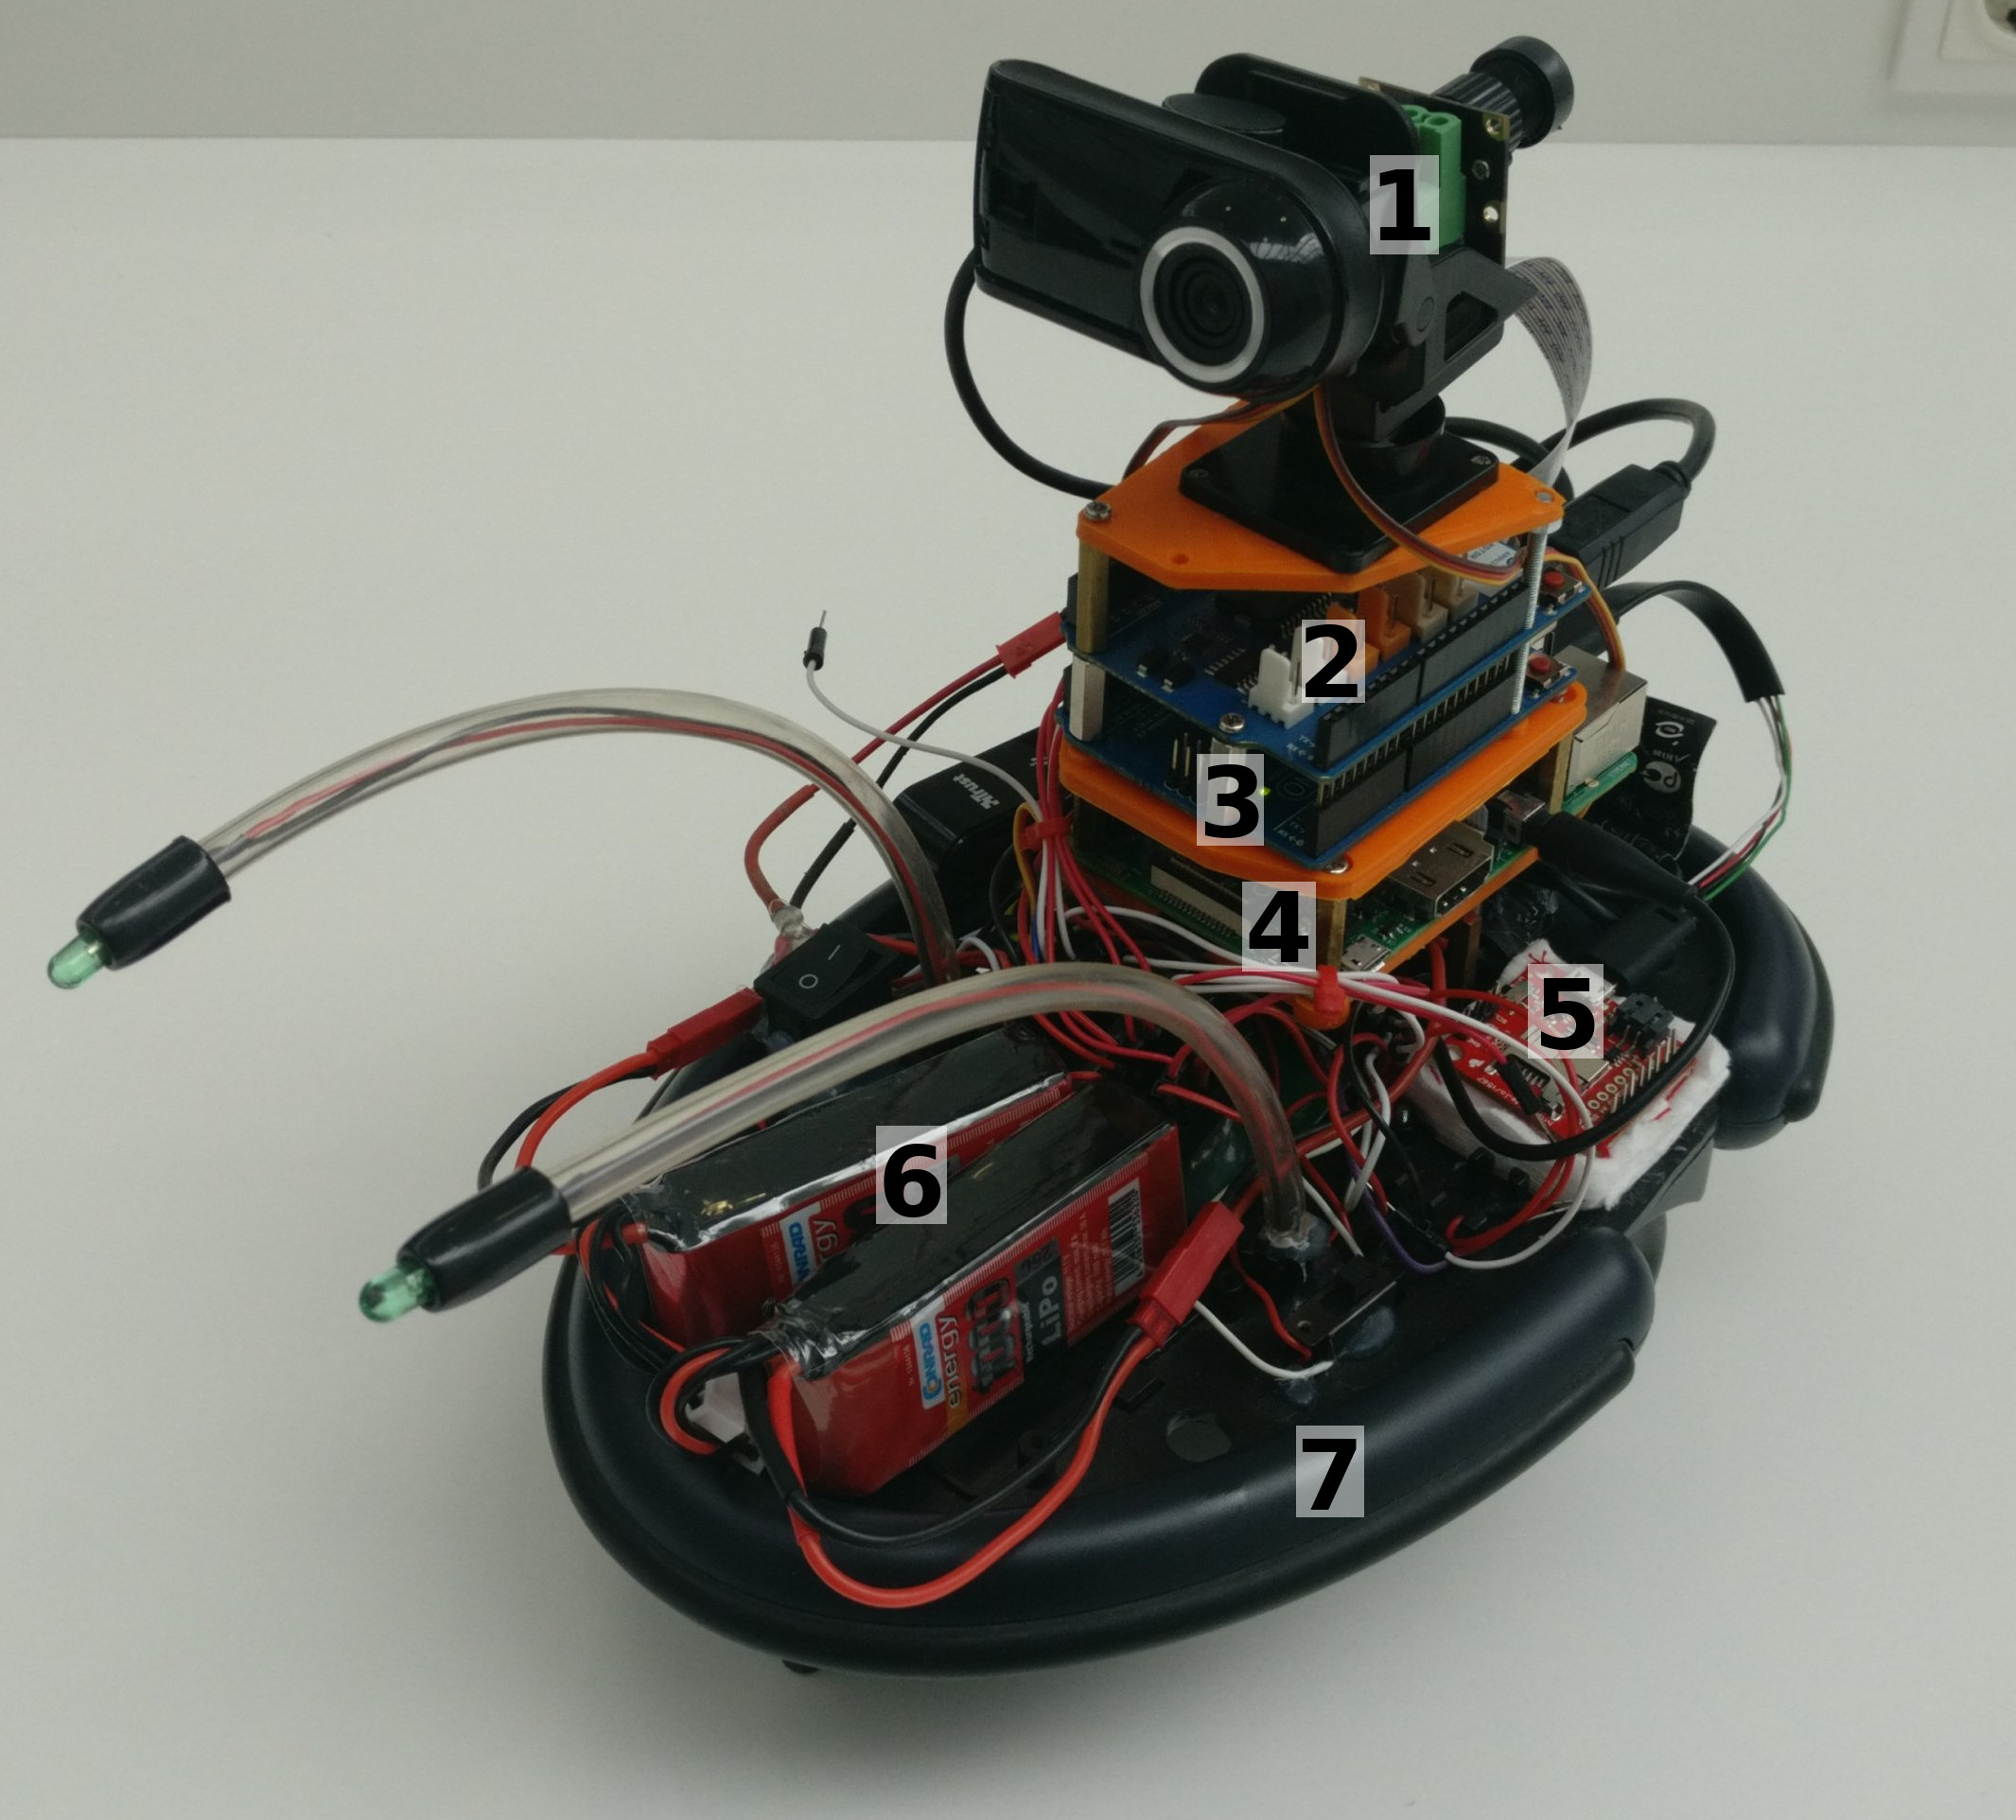
\includegraphics[width=8cm]{images/profile_numbered}
 \captionsetup{singlelinecheck=off}
 \caption[]{
  Here is an overview of all the components:
  \begin{enumerate}
   \item Raspberry Pi Night Vision Camera Module and Logitech C905 Webcam
   \item Arduino Motor Shield Rev 3
   \item Arduino Uno Rev 3
   \item Raspberry Pi 3 Model B Rev 1.2
   \item SparkFun 9DoF Razor IMU M0
   \item 2x 1000 mAh batteries with a 5V voltage regulator
   \item Cybot chassis, motors and other remains
  \end{enumerate}
 }
 \label{fig:platform}
\end{figure}

An exact cost of the platform is hard to determine, because many of the parts were either scraps or were freely available to use for this project. We estimate a sub 200\$ for all the parts used if bought new.

\begin{center}
    \begin{figure}
\begin{tikzpicture}[align=center,node distance=3cm]
    \node[block] (lipo1) {11.1V LiPo};

    \node[block] (regulator) [right of=lipo1] {5V regulator};

    \node[block] (rpi) [right of=regulator] {RPI};
    \node[block] (imu) [right of=rpi] {IMU};
    \node[block] (cameras) [above of=rpi] {Cameras};
    \node[block] (arduino) [below of=rpi] {Arduino};
    \node[block] (motorshield) [below of=arduino] {Motor Shield};
    \node[block] (motors) [right of=motorshield] {DC motors};
    \node (empty1) [below of=lipo1] {};
    \node[block] (lipo2) [below of=empty1] {11.1V LiPo};

    \draw[-] (rpi.south) -- (arduino.north);
    \draw[-] (arduino.south) -- (motorshield.north);
    \draw[-] (motorshield.east) -- (motors.west);
    \draw[-] (rpi.east) -- (imu.west);
    \draw[-] (rpi.north) -- (cameras.south);

    \draw[dashed] (lipo1.east) -- (regulator.west);
    \draw[dashed] (regulator.east) -- (rpi.west);
    \draw[dashed] (lipo2.east) -- (motorshield.west);


\end{tikzpicture}
\caption{Block diagram of the hardware layout}
\end{figure}
\end{center}

\vspace{1cm}

\subsection{Embedded Computing}\label{subsec:soc}
\pagestyle{scrheadings}

We built our platform around the Raspberry Pi 3 Model B. Its low cost, computational performance, availability, low power consumption and ROS support made it a clear choice.

The Raspberry Pi is a single board computer(SBC) with a Broadcom BCM2837 system on chip(SoC) that has a Quad-Core ARM Cortex-A53 and a Broadcom VideoCore IV. It has 1GB of LPDDR2 memory. For communication it has Bluetooth, Wifi and 10/100 Mbit Ethernet, 40 GPIO pins, display serial interface(DSI), camera serial interface(CSI) and 4 USB ports\footnotemark.

\footnotetext{https://www.raspberrypi.org/magpi/raspberry-pi-3-specs-benchmarks/}

The Raspberry Pi is connected to an Arduino Uno via a USB and the Arduino Uno is connected to an Arduino Motor Shield. Therefore any Arduino compatible sensors or actuators can be easily integrated onto the platform.

\subsection{Chassis}\label{subsec:chassis}
\pagestyle{scrheadings}

The chassis and most of the plastic parts were taken from the Cybot, a toy robot that came with the magazine Real Robots by Eaglemoss Publications\footnotemark.

\footnotetext{https://www.getreading.co.uk/news/local-news/make-your-robot-home-4278122}

In order to securely stack the boards, plates were 3D printed and mounted between the Raspberry Pi and the chassis, Arduino and Raspberry Pi, the Arduino Motor Shield and camera stand.

\subsection{Actuators}\label{subsec:actuators}
There are two generic 12V DC motors that were left in from the Cybot. They are mounted under the base plate and are connected to the wheels with a plastic gearbox. The Arduino Motor Shield supplies them with 11.1V and can reverse the polarity to turn in both directions.

\subsection{Sensors}\label{subsec:sensors}
There are two cameras on the top of the robot facing away from each other, providing almost full 360 degrees of field of view. The Logitech Webcam is connected via USB and the Camera Module via camera serial interface(CSI) to the Raspberry Pi.

As for an inertial measurement unit(IMU) we first deployed an MPU6050 and was connected through $ I^2C $ on the Raspberry Pi, but because of driver issues we went with a 9DoF Razor IMU M0, which is an all in one solution fully supported by ROS.

\subsection{Power management}\label{subsec:power}
To ensure adequate longer mobility, two 1000 mAh LiPo batteries were used: One of them distributes power to the actuators, while the other to the sensors and boards. This was done for additional voltage stability, since the motor movement causes additional noise and spikes which will interfere with our sensors. For easy plug and play a power distributing board was made from the boards of the Cybot and secured with hot glue. Since the LiPo batteries voltage is 11.1V, the conversion to 5V is handled by a voltage regulator.

\end{document}
